%%%%%%%%%%%%%%%%%%%%%%%%%%%%%%%%%%%%%%%%%%%%%%%%%%%%%%%%%%%%%%%%%%%%%%%%%%%%%%%%%%%%%%%%%%%%%%%%%%%%%%%%%%%%%%%%%%%%%%%%
\newpage
\chapter {\Large{Siminov ORM Architecture}}

\begin{figure}[!htbp]
	\centering
		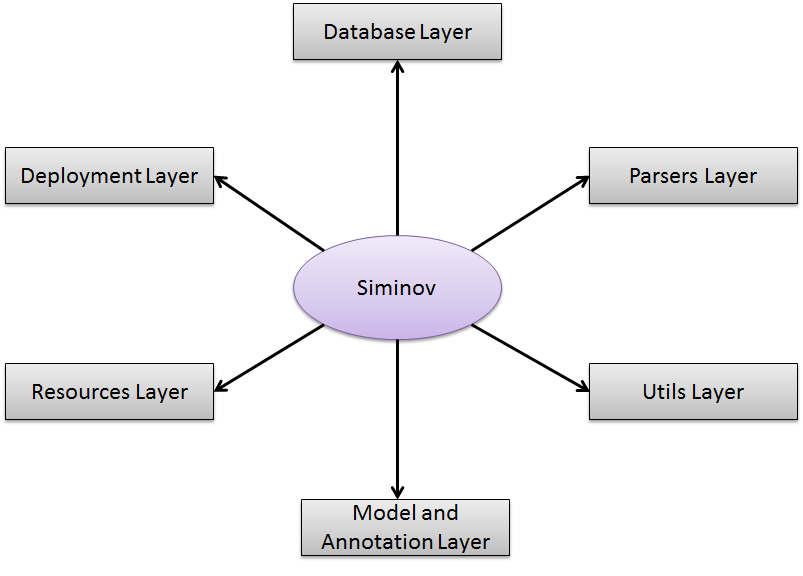
\includegraphics[height=8cm]{Resources/siminov_layers.png}
	\caption{Siminov ORM Layers}
\end{figure}


\newpage
\section{Deployment Layer}
When application starts for first time it does not have its database's. Siminov provides deployment layer, it creates application database's by reading all descriptors from application assests and its libraries.

\textbf{\subsection{siminov.orm.Siminov}}

		\lstinputlisting[language=Java]{Resources/siminov_class.txt}


\newpage
\section{Resources Layer}
It holds meta data about application needed by Siminov. 

\textbf{\subsection{siminov.orm.Resources}} Only GET APIS shown, for rest visit Javadoc
		\lstinputlisting[language=Java]{Resources/resources_class.txt}


\newpage
\section{Database Layer}
This layer basically deals with database operations.

\textbf{\subsection{siminov.orm.database.Database}}
	
		\lstinputlisting[language=Java]{Resources/database_class.txt}


\newpage
\section{Model and Annotation Layer}
It holds Model POJO classes and Annotation defination required for database mapping descriptor.


\textbf{\subsection{siminov.orm.model.ApplicationDescriptor}}

	
		\lstinputlisting[language=Java]{Resources/application_descriptor_class.txt}
		
\newpage
\textbf{\subsection{siminov.orm.model.DatabaseDescriptor}}

		\lstinputlisting[language=Java]{Resources/database_descriptor_class.txt}

	
\newpage
\textbf{\subsection{siminov.orm.model.LibraryDescriptor}}

		\lstinputlisting[language=Java]{Resources/library_descriptor_class.txt}


\newpage
\textbf{\subsection{siminov.orm.model.DatabaseMappingDescriptor}}

		\lstinputlisting[language=Java]{Resources/database_mapping_descriptor_class.txt}


\newpage
\textbf{\subsection{siminov.orm.annotation.Table}}

		\lstinputlisting[language=Java]{Resources/table_annotation_interface.txt}

	
\newpage
\textbf{\subsection{siminov.orm.annotation.Column}}

		\lstinputlisting[language=Java]{Resources/column_annotation_interface.txt}

	
\newpage
\textbf{\subsection{siminov.orm.annotation.Property}}

		\lstinputlisting[language=Java]{Resources/properties_annotation_interface.txt}

\newpage
\textbf{\subsection{siminov.orm.annotation.Index}}

		\lstinputlisting[language=Java]{Resources/index_annotation_interface.txt}

\newpage
\textbf{\subsection{siminov.orm.annotation.IndexColumn}}

		\lstinputlisting[language=Java]{Resources/index_column_annotation_interface.txt}

	
\newpage
\textbf{\subsection{siminov.orm.annotation.Indexes}}

		\lstinputlisting[language=Java]{Resources/indexes_annotation_interface.txt}


\newpage
\textbf{\subsection{siminov.orm.annotation.Reference}}

		\lstinputlisting[language=Java]{Resources/reference_annotation_interface.txt}


\newpage
\textbf{\subsection{siminov.orm.annotation.Map}}

		\lstinputlisting[language=Java]{Resources/map_annotation_interface.txt}


\newpage
\section{Parsers Layer}
It contain parses which parses all descriptor defined by application.


\textbf{\subsection{siminov.orm.parsers.ApplicationDescriptorParser}}
It is used to parse ApplicationDescriptor.si.xml files defined by application.
	
\textbf{\subsection{siminov.orm.parsers.DatabaseDescriptorParser}}
It is used to parse DatabaseDescriptor.si.xml files defined by application.
	
\textbf{\subsection{siminov.orm.parsers.LibraryDescriptorParser}}
It is used to parse LibraryDescriptor.si.xml files defined by application.
	
\textbf{\subsection{siminov.orm.parsers.DatabaseMappingDescriptor}}
It is used to parse DatabaseMappingDescriptor.si.xml files defined by application.


\newpage
\section{Utils Layer}
It provides util classes which provides additional befinites.

\textbf{\subsection{siminov.orm.utils.Utils}}

		\lstinputlisting[language=Java]{Resources/utils_class.txt}

